%!TEX root = ../main.tex
% mainfile: ../main.tex

\section{Experiments}
\subsection{Dataset Description}

The study described in this chapter uses two datasets: (i)
a gold standard report (GSR) of social unrest events in Latin America
provided by MITRE that we use to define
major mass protest events, and (ii)
tweets collected over 14 months from May 2012 to September 2013 from 20
Latin American countries.

The GSR documents each civil unrest event by location, date, type
of protest, and specifies the national news articles that
first reported the event. For protests that were prominent on Twitter, the
GSR news articles often report hashtags which were used by protestors
on social media. We selected only those GSR events for which we
were able to find such hashtags. This process resulted in 64
unique hashtags related to 40 different protest that occurred
in Latin America since May 2012. In Table 1 we list a few of
these events from our study.

Our Twitter dataset was built by querying Datasift's streaming API. Each tweet payload includes crucial metadata along with the tweet's content. Though tweets from GPS-enabled devices include geographic coordinates, the percentage of such tweets in the collected sample was too low to be useful.

For this study, we further filtered tweets by removing those that do not contain hashtags relevant to a specific protest. Since most tweets do not have location data, we estimate their location by geocoding the tweet based on each tweet's content and properties of its user. We developed our own geocoding library that uses the World Gazetteer (http://archive.is/srm8P) database to lookup location names and geographic coordinates. Tweets can be geocoded to the user's location at the time of tweeting or a location of interest about which the user is tweeting. We focused on event geolocation, which looks for location or landmark names, such as \textit{Plaza de la Independencia} or \textit{Quito, Ecuador}, in a tweet's text.  We generated a list of 2000 landmarks by extracting place names mentioned in GSR events which had high mutual information to civil unrest. In cases where no event location was found in a tweet's text, we use geo-coordinates or self-reported location string in the tweet's metadata.

Using the above pipeline we were able to extract and geolocate $20,227,830$ unique users to build our mentions network from the filtered tweets that were spread over daily sub-networks.


\begin{figure}[t]
\centering
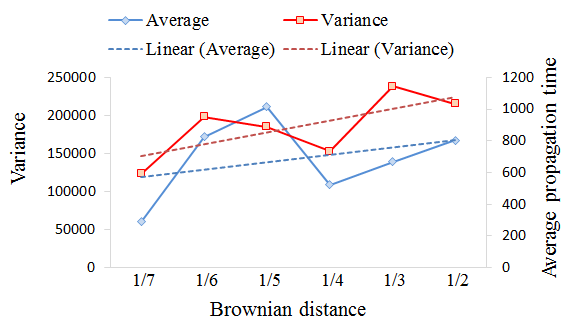
\includegraphics[width=3.5in] {figures/infectdTime.png}
\caption{Brownian distance vs propagation time
for teacher protest events.}
\label{fig:timecurve}
\end{figure}




\begin{figure}[t]
\centering
\subfigure[Simulation without community]{
   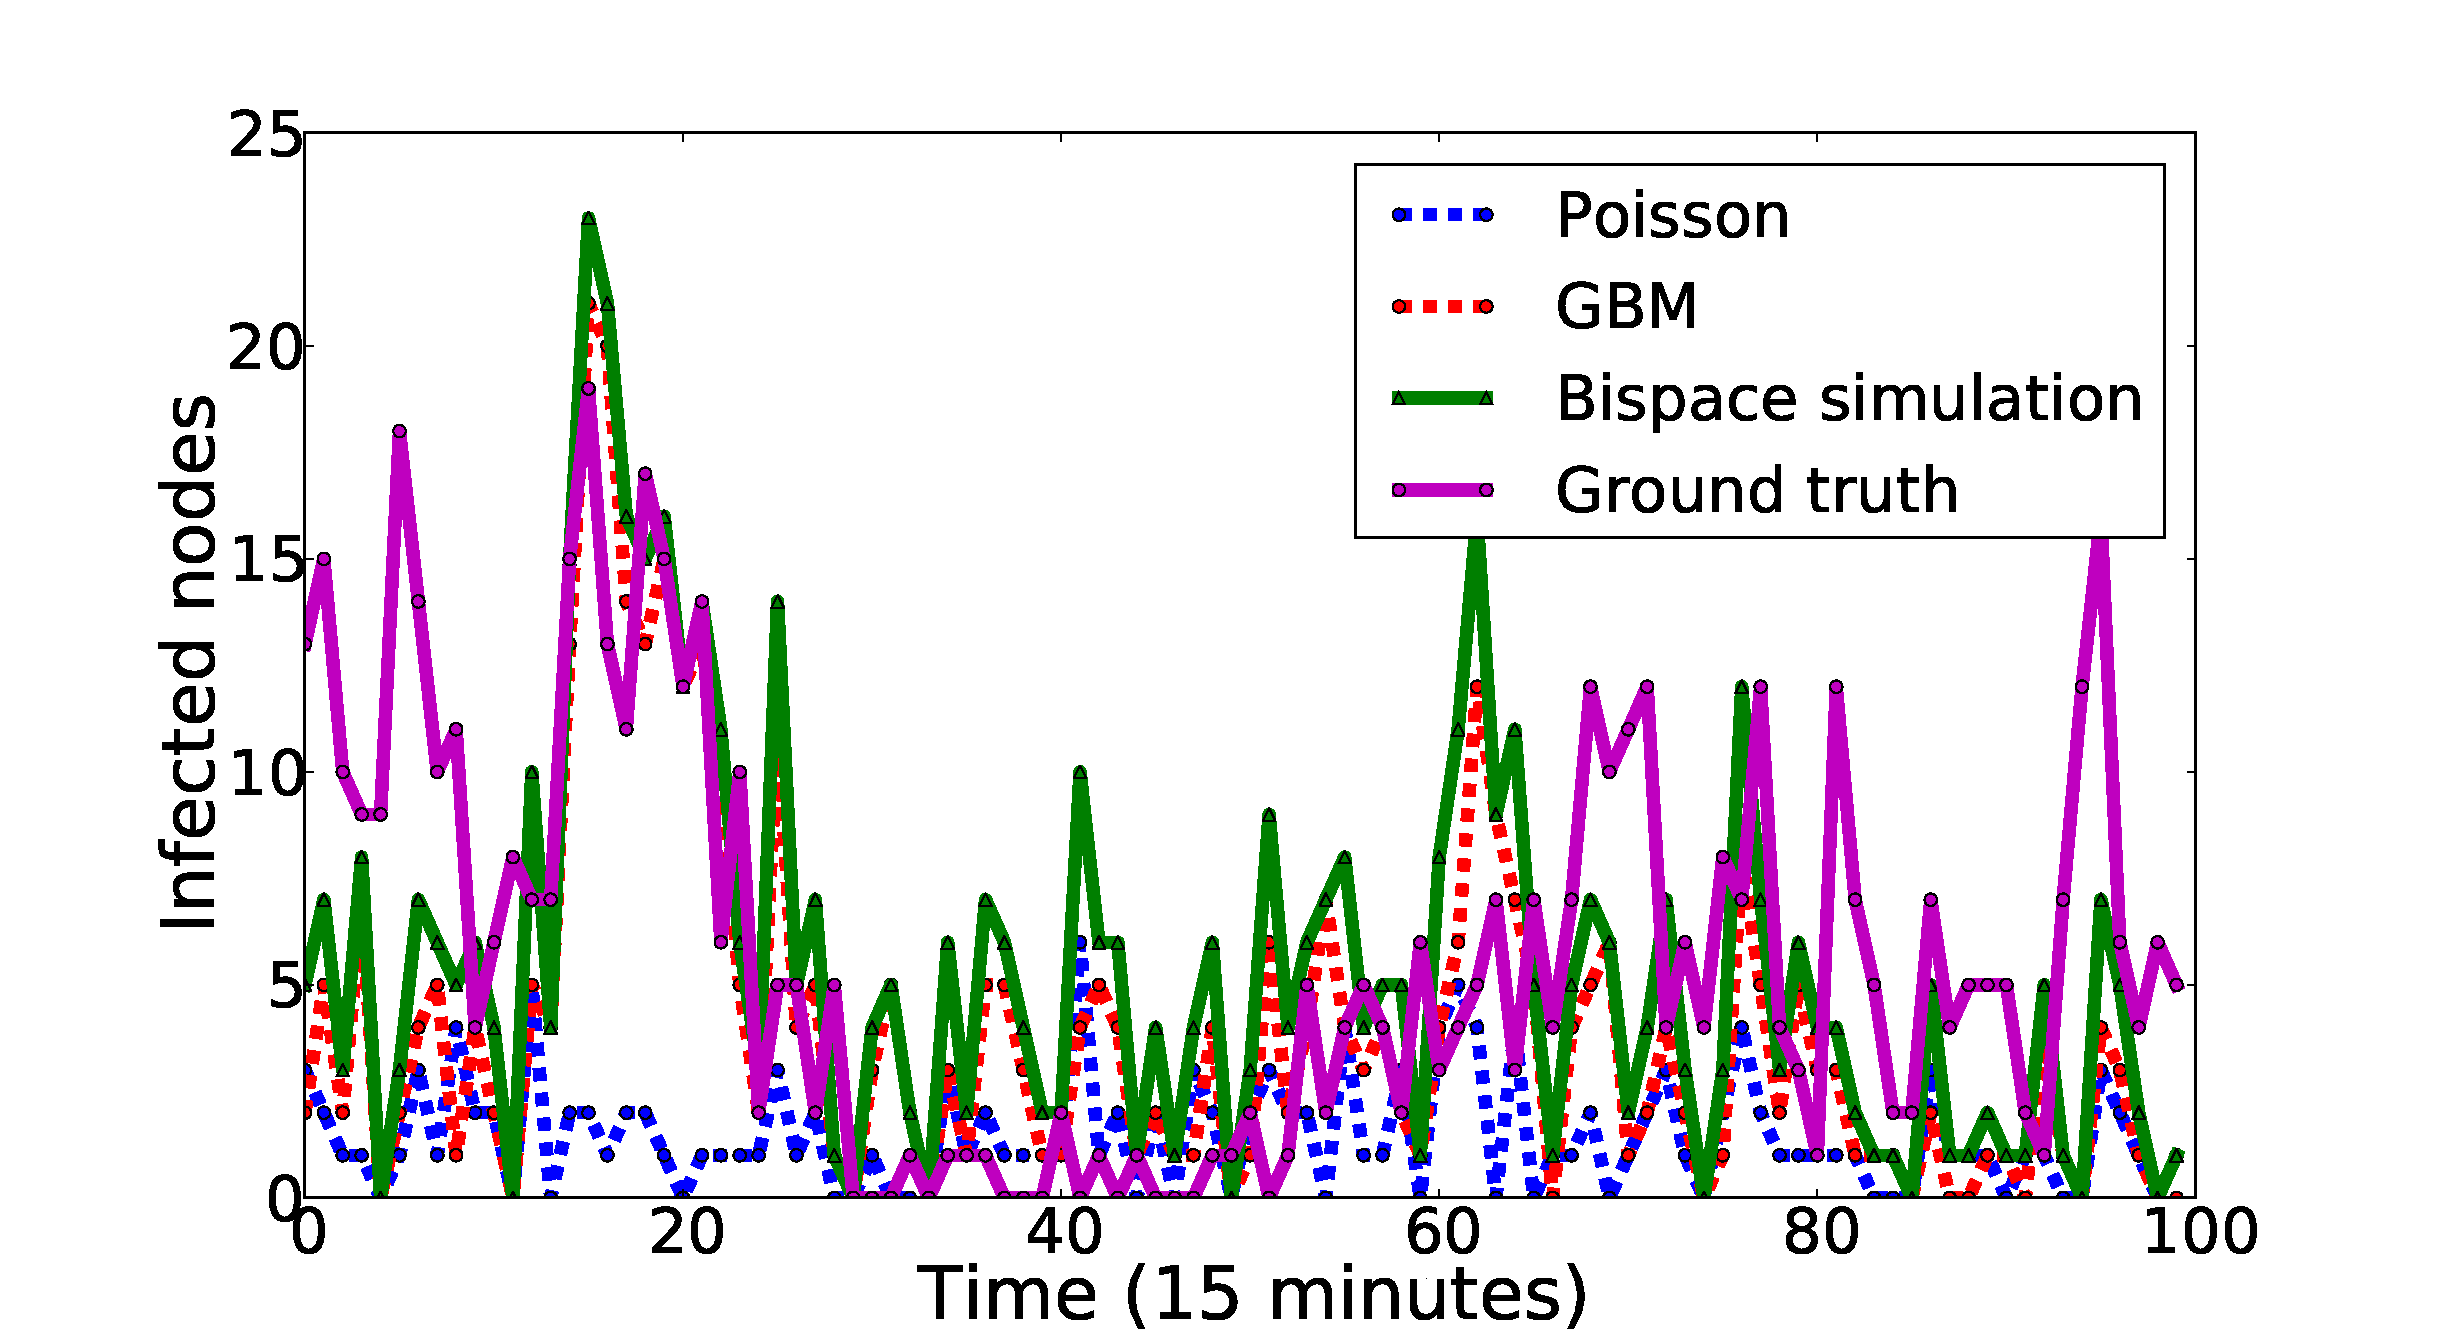
\includegraphics[width=3in,height=1.6in] {figures/1-yosoy-without-community-final.pdf}
  \label{fig:yosou_no_community}
 }
 \subfigure[Simulation with community]{
   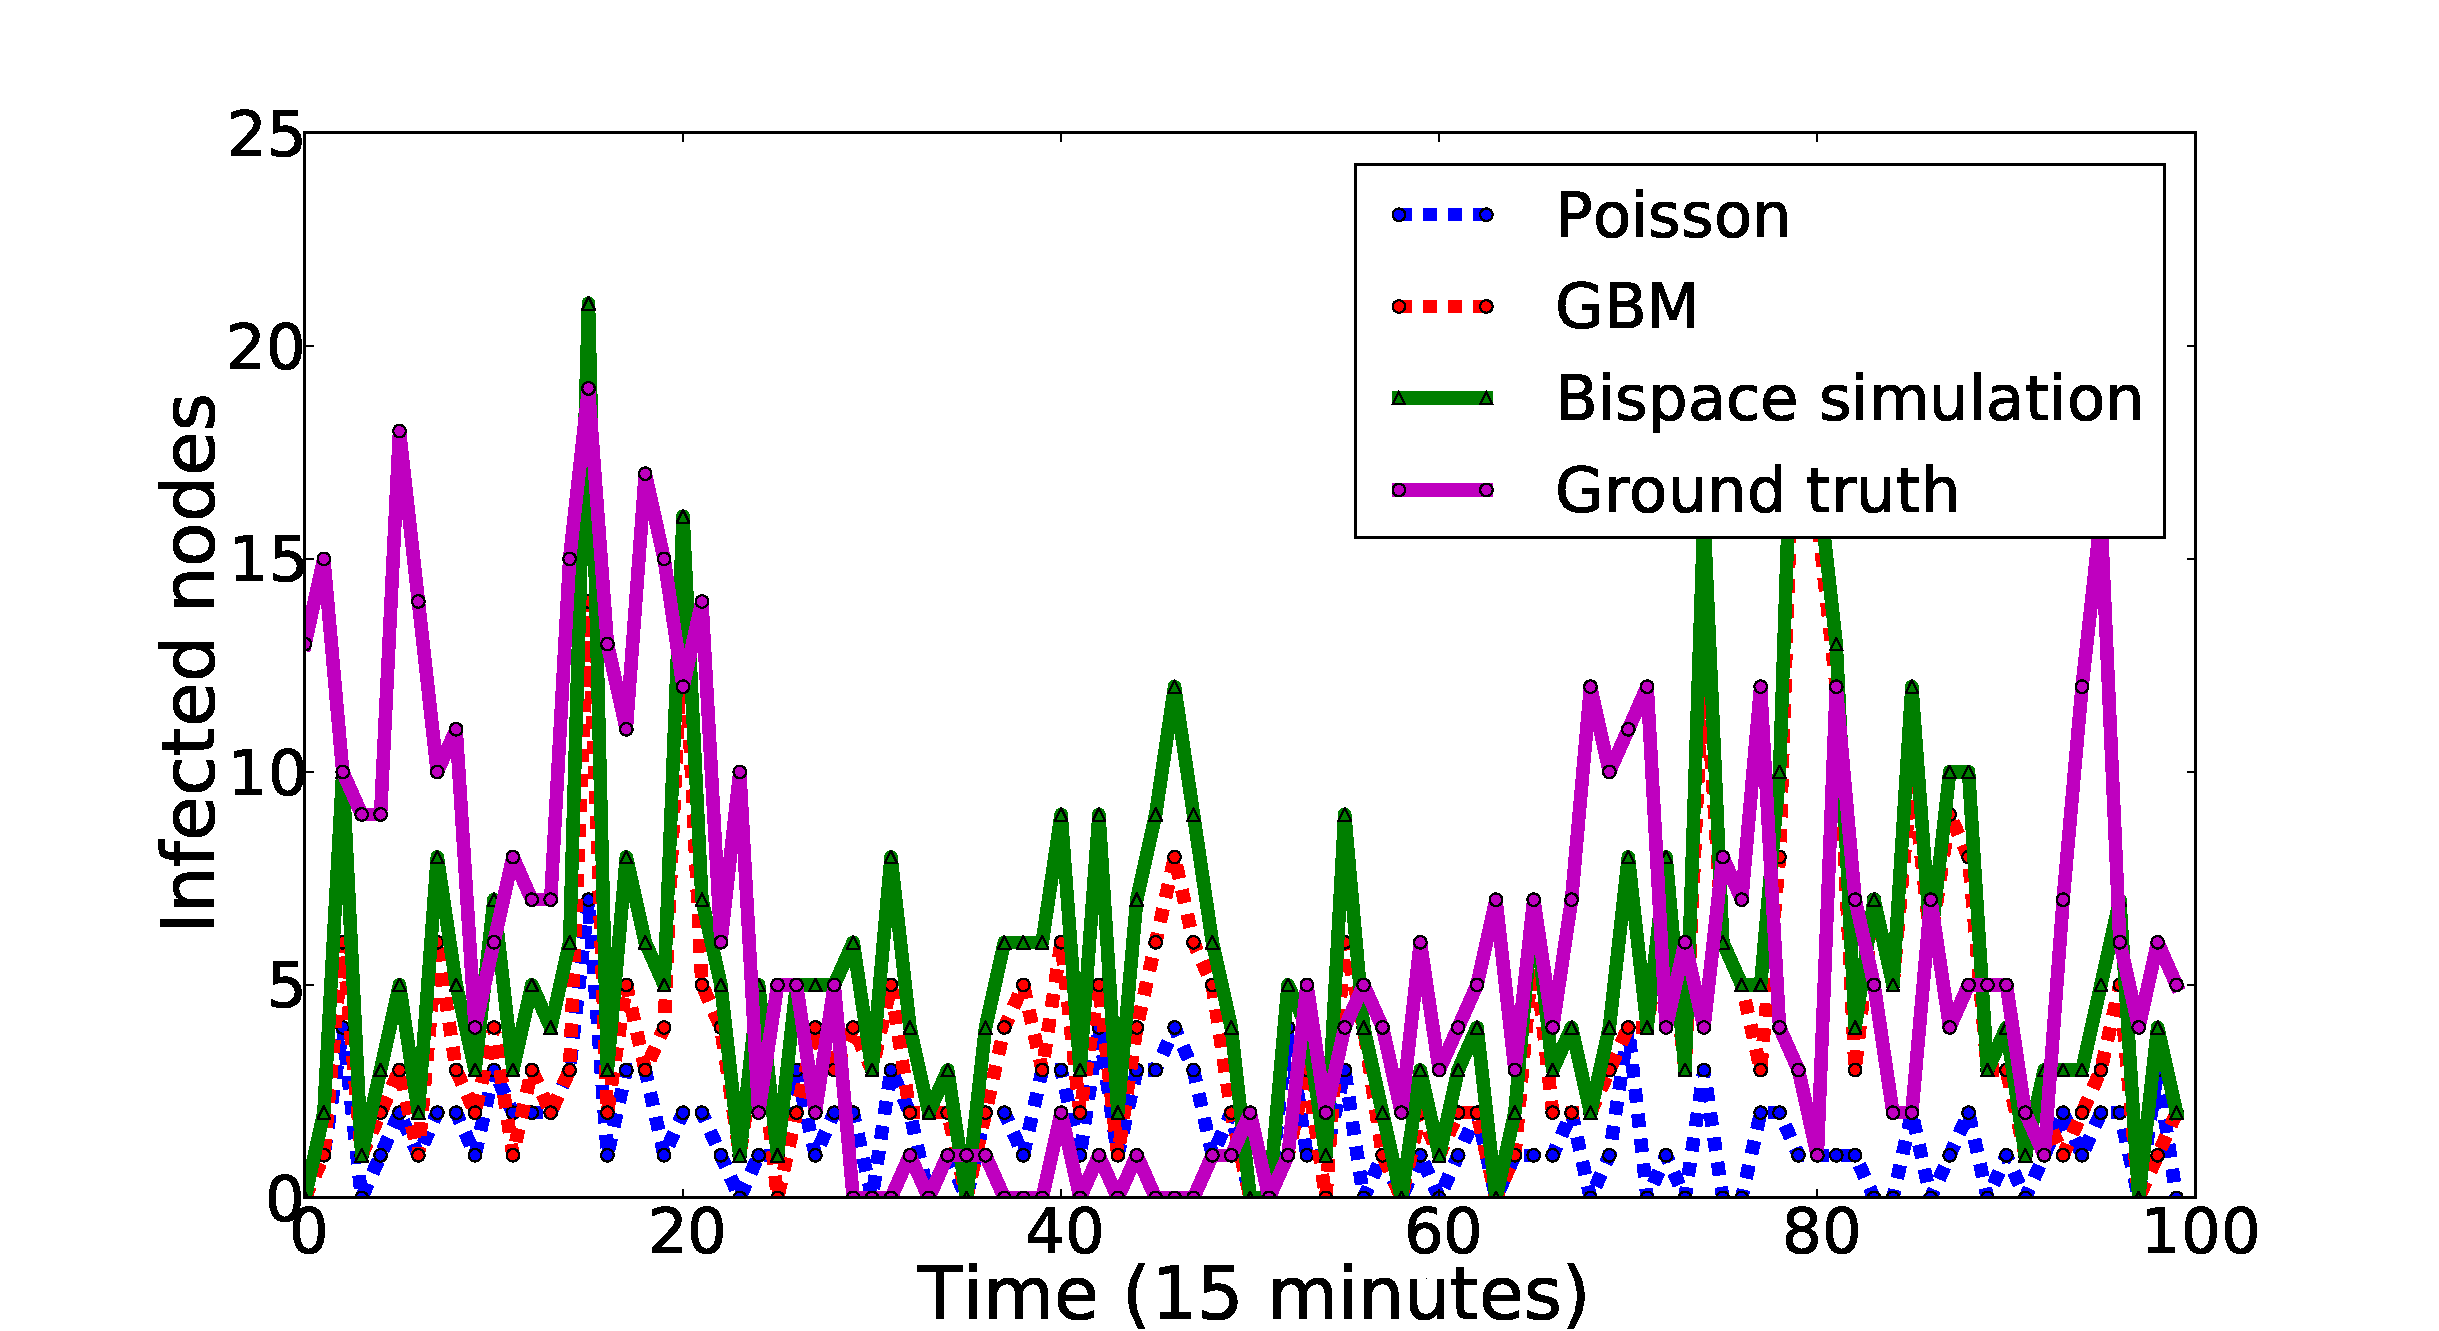
\includegraphics[width=3in,height=1.6in] {figures/1-yosoy-with-community-final.pdf}
  \label{fig:yosou_community}
 }
\caption{GBM and Poisson propagation simulation for Yosoy protests
(Mexico) on May 19, 2012.}
\label{fig:1Yosoy2012may}
\end{figure}


\begin{figure}[th]
\centering
\subfigure[Simulation without community]{
   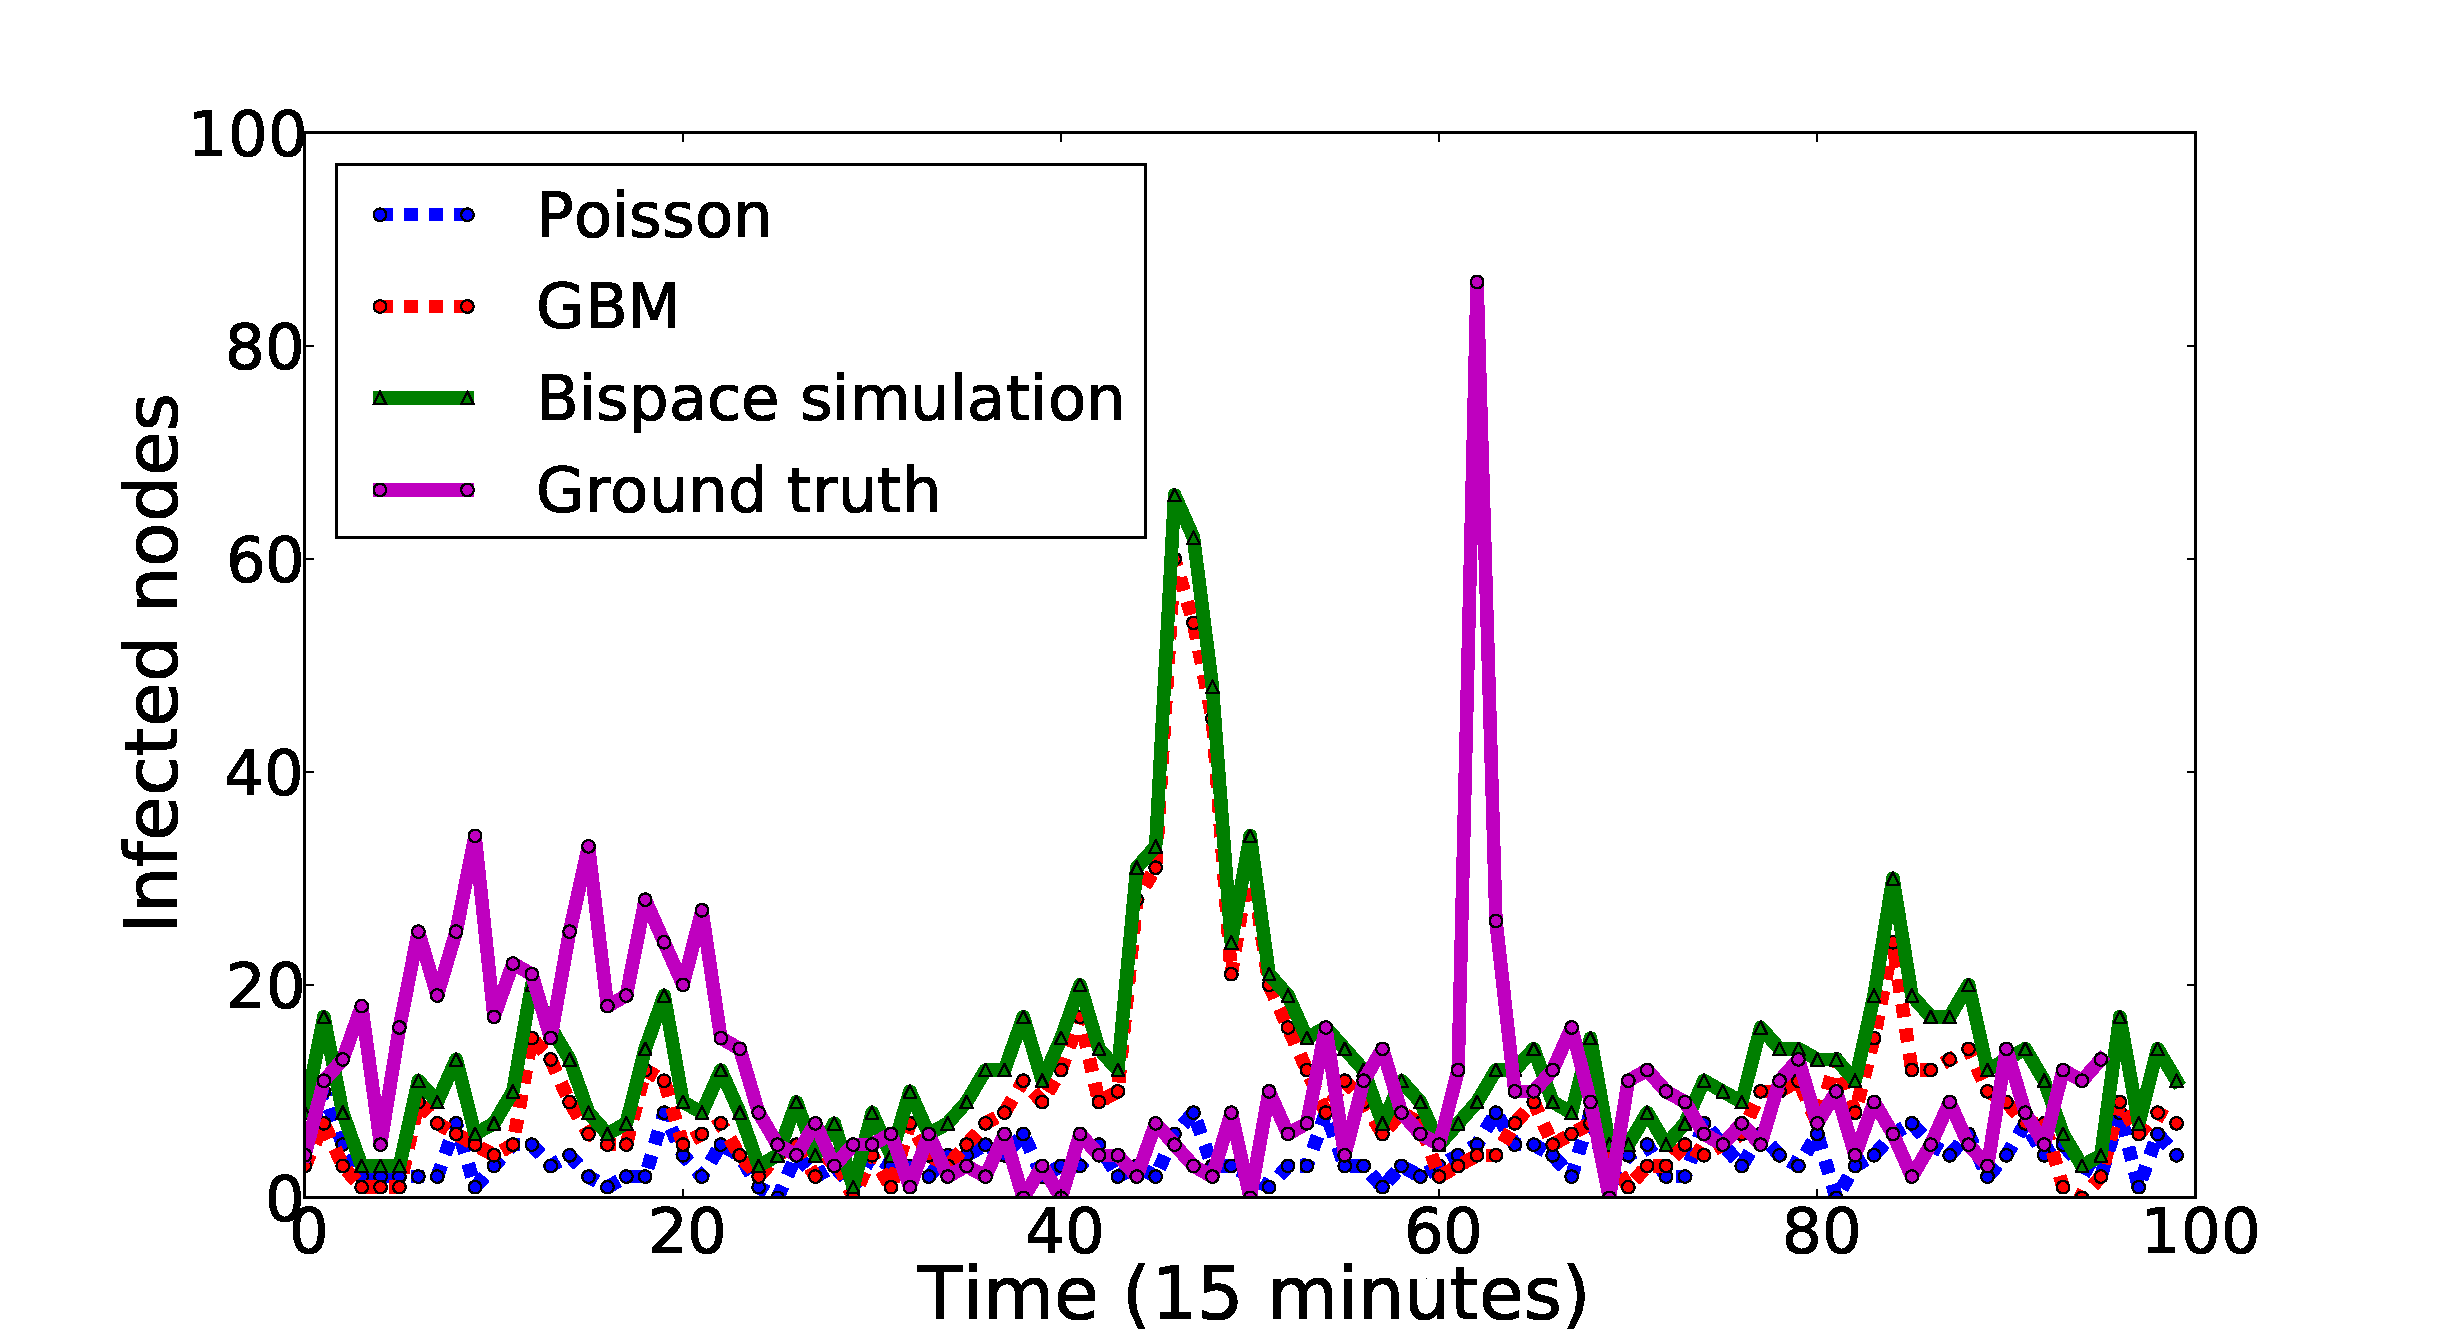
\includegraphics[width=3in,height=1.6in] {figures/4-teacher-without-community-final.pdf}
  \label{fig:teacher_no_community}
 }
 \subfigure[Simulation with community]{
   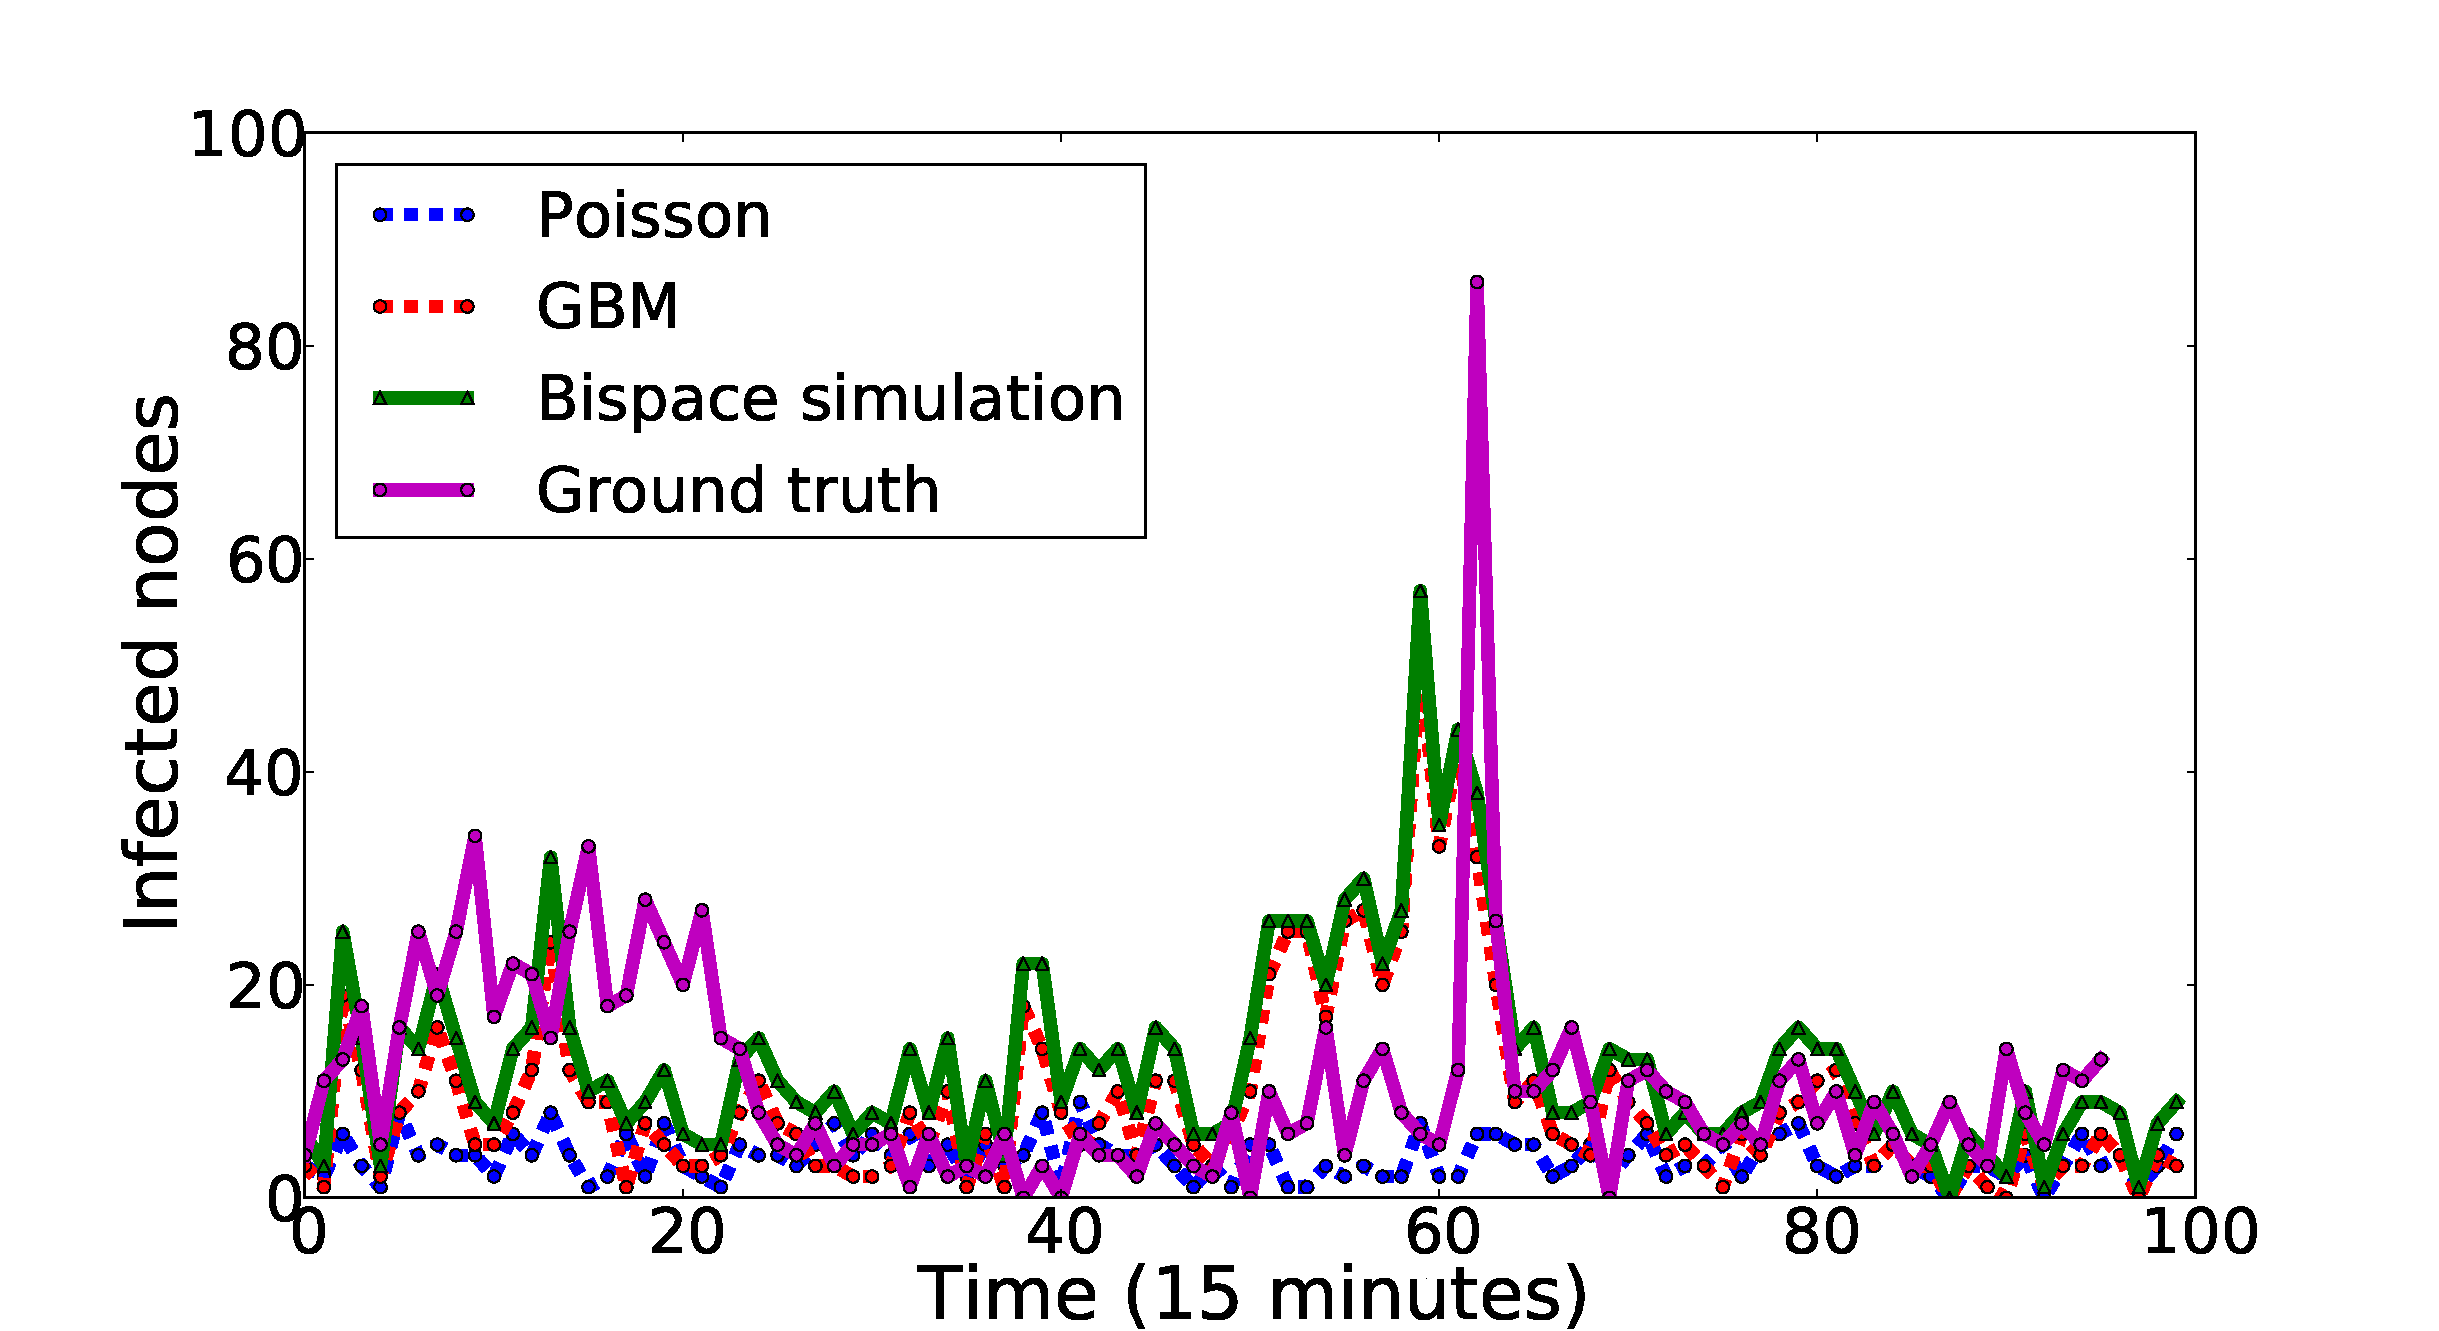
\includegraphics[width=3in,height=1.6in] {figures/4-teacher-with-community-final.pdf}
  \label{fig:teacher_community}
 }
\caption{GBM and Poisson propagation simulation for teacher protests (Mexico)
on Sep 1, 2013.}
\label{fig:4teacherSimulation}
\end{figure}


\begin{figure}[th]
\centering
\subfigure[Simulation without community]{
   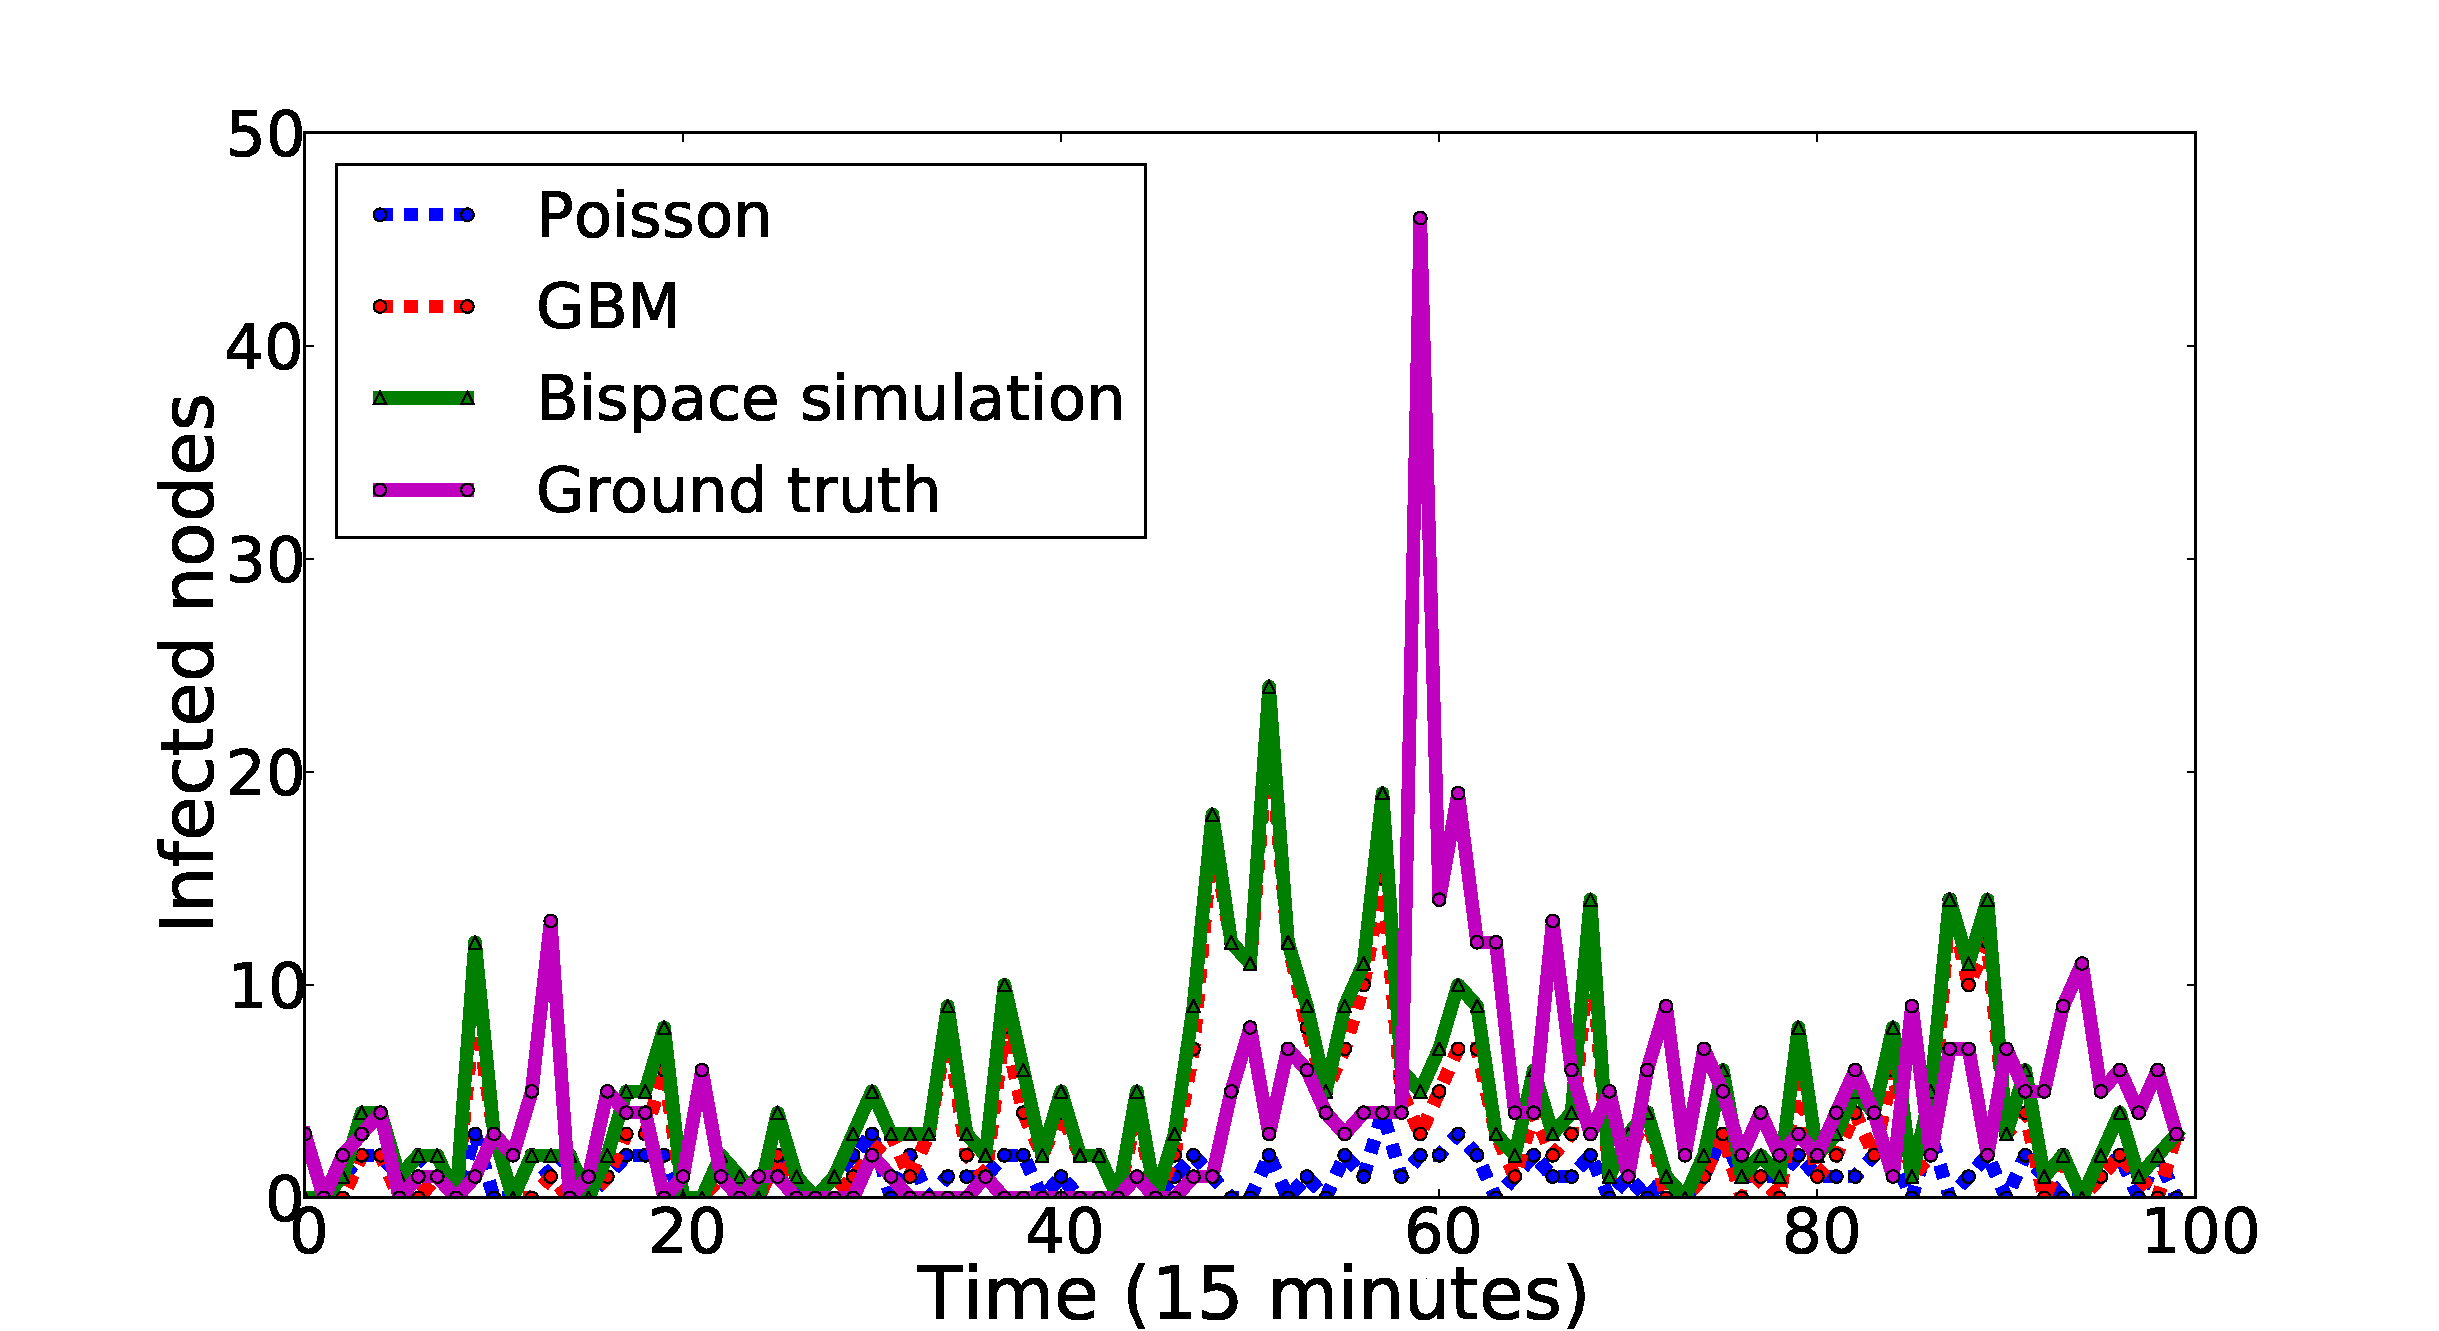
\includegraphics[width=3in,height=1.6in] {figures/7-colombia-without-community-final.pdf}
  \label{fig:colombia_no_community}
 }
 \subfigure[Simulation with community]{
   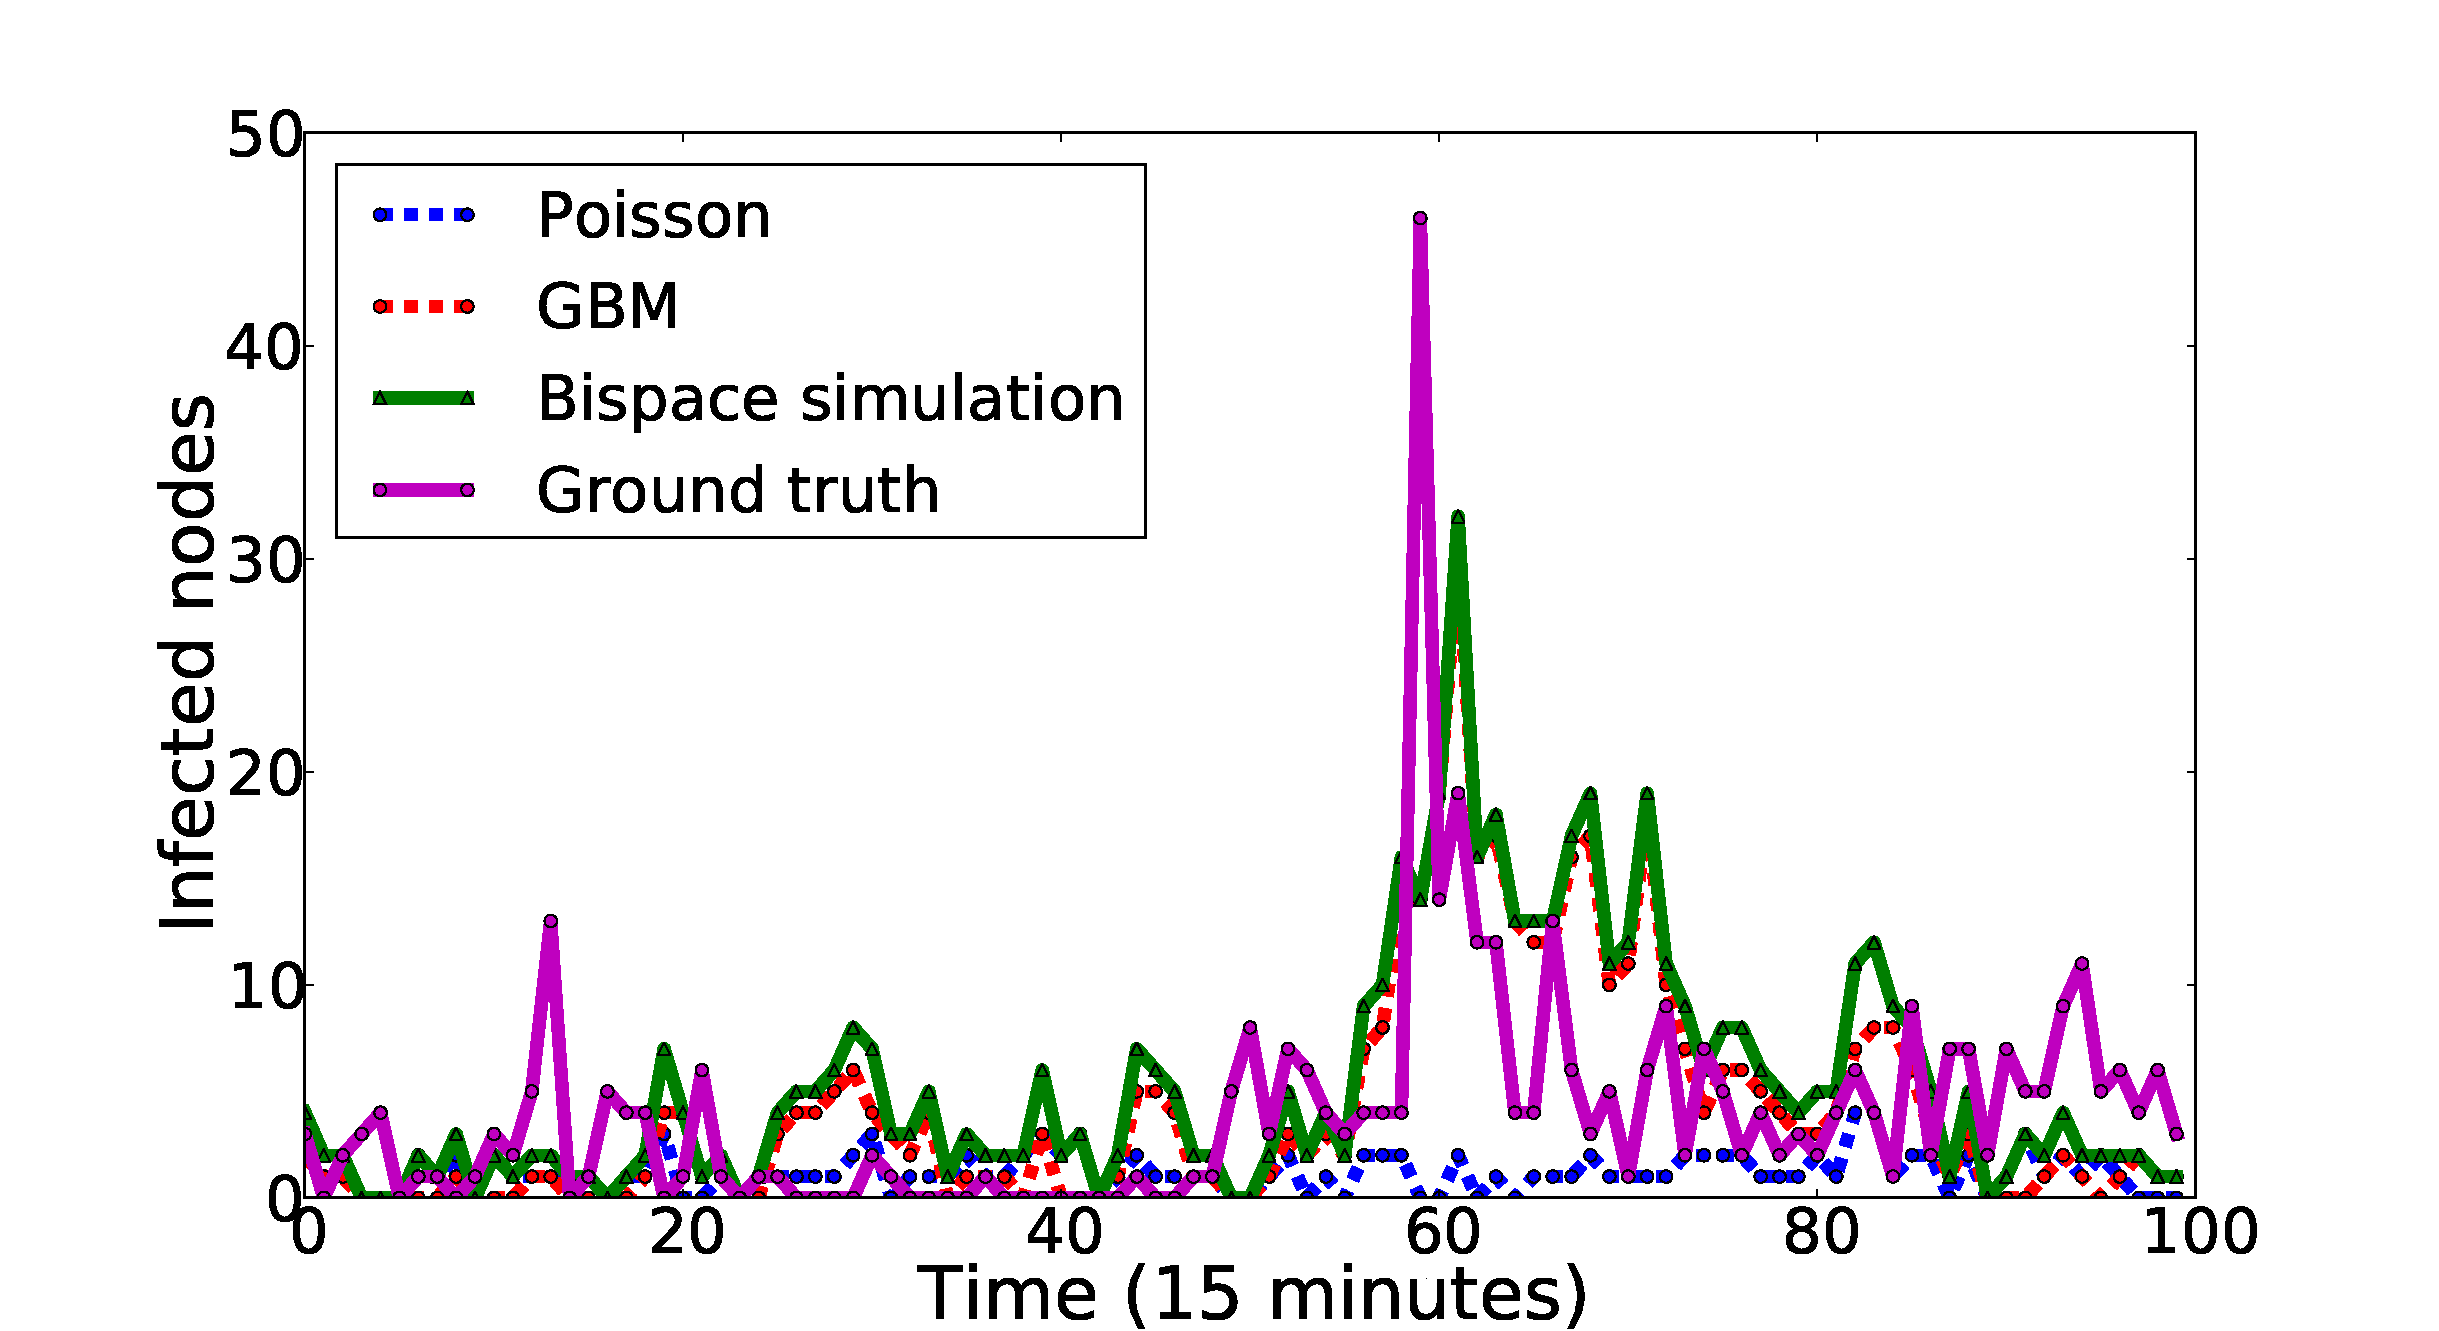
\includegraphics[width=3in,height=1.6in] {figures/7-colombia-with-community-final.pdf}
  \label{fig:colombia_community}
 }
\caption{GBM and Poisson propagation simulation for Colombia protests on Dec 4, 2012.}
\label{fig:7ColombiaProtest}
\end{figure}




\subsection{GBM Diffusion Model}
For each of our mass protest events, we filter by its specific keywords (hashtags) to obtain a set of relevant tweets and construct a mentions network from those tweets. We assume that information propagates from an initial infected user to other users through the network from one node to its neighbors. We build an adjacency matrix based on the mentions network and simulate the propagation using the GBM diffusion process as follows:
\begin{enumerate}
  \item \textbf{Brownian distance:} The Brownian distance is intended to have
an inverse relationship with mention frequency. As Fig.~\ref{fig:timecurve} shows, users with smaller Brownian distance have greater mention frequencies resulting in shorter mean propagation times with less variance. From Fig.~\ref{fig:timecurve}, we can see that infection time and variance generally both increase with an increase in Brownian distance. Heuristically, more frequent mentions indicate stronger ties which leads to easier adoption of information.

  \item \textbf{Propagation speed: } To evaluate our dynamic GBM
infection process assumptions, we estimate the GBM parameters for different protest events and depict the GBM propagation curves in Figs.~\ref{fig:1Yosoy2012may},~\ref{fig:4teacherSimulation}, and~\ref{fig:7ColombiaProtest}. The blue curve depicts the Poisson propagation in latent space. The red curve depicts GBM propagation through the mentions network. The green curve is the overall simulation result while the magenta curve depicts the ground truth of the protest events process. By comparing the green and magenta curves, we can evaluate the
effectiveness of our bispace model in simulating the mass protest events.
As shown, we find that, given a mentions network, our bispace model can simulate the propagation speed at a reasonable scale, at the right magnitudes. As seen in Figs.~\ref{fig:yosou_no_community},~\ref{fig:teacher_no_community} and~\ref{fig:colombia_no_community},
we find that we can capture the burst of activity at the same time point as the ground truth during protest propagation.


\end{enumerate}



\begin{figure}[ht]
\centering
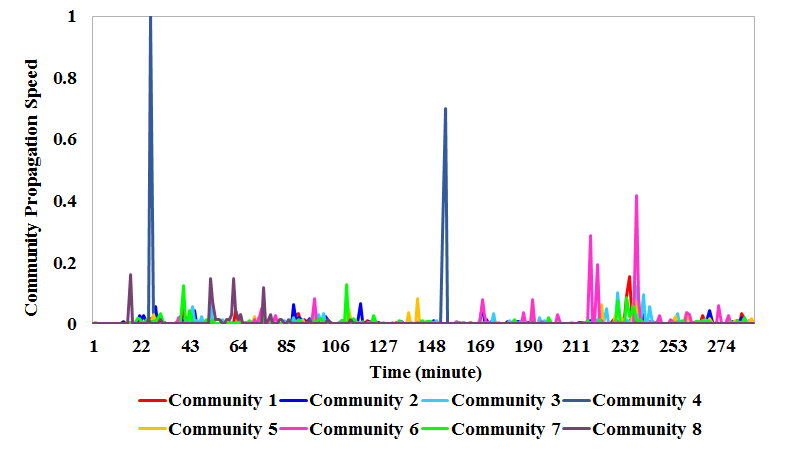
\includegraphics[width=4.5in] {figures/4teacher-community-speed.png}
\caption{Normalized mass-protest propagation speed for major communities during teacher protest events.}
\label{fig:teacher_community_speed}
\end{figure}



\subsection{GBM Diffusion with Communities}
We were also able to observe the variation in $\mu$ and $\sigma$ as community structure varies. In particular, community features like graph density and diameter as shown earlier in Fig.~\ref{fig:teacher_community_parameters0} may impact GBM propagation.
%To illustrate the relationship between the GBM parameter $\mu$ and graph structure, we plot $\mu$ against diameter and density for several communities in Figure~\ref{fig:density_diameter}. We can see the larger of a community diameter, the higher of propagation parameter $\mu$, while the smaller of graph density, the higher of propagation parameter $\mu$.
We experimented with two modeling approaches: (i) one set of parameters for the whole network and (ii)
different parameters
for each community in the network.
We ran simulations for both these situations,
and plotted the results of the whole network vs. community-specific approach in Figs.~\ref{fig:1Yosoy2012may},~\ref{fig:4teacherSimulation}, and~\ref{fig:7ColombiaProtest}.
Comparing these simulation results, we find the community approach performs better, especially at capturing peak values. Taking a closer look at Fig.~\ref{fig:teacher_community_speed}, we observe that propagation time and speed of infection are different for each community and we are able to simulate local propagation more accurately, which can be seen, e.g.,
from Fig.~\ref{fig:teacher_community}, where
the GBM with community method can simulate the burst
propagation effectively, while the general GBM method (see Fig.~\ref{fig:teacher_no_community}) fails to capture the exact peak time.


\begin{figure}[ht]
\centering
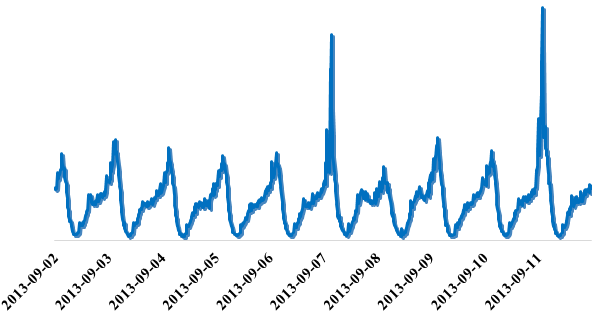
\includegraphics[width=3.5in] {figures/Baseline.png}
\caption{Total tweets over time from Sep 2 to Sep 11, 2013 (Mexico).}
\label{fig:Baseline}
\end{figure}

\subsection{Latent Space Diffusion Model}
We use the following steps to calculate the properties of the latent space for each event.

\begin{enumerate}
  \item \textbf{Latent space:} The intent is
to consider all possible external influences and latent interactions in this space. We split Twitter data into unique 15 minute intervals and count the total
number of infected users in each interval.
  \item \textbf{Normalize:} Twitter user activity varies based on time of day and day of week (see Fig.~\ref{fig:Baseline}). For each 15 minute window from Step 1, we find the average number of tweets over a 4 week period and use this value to normalize the count. This baseline count of tweets over time in the latent space is close to the Poisson distribution.
  Fig.~\ref{fig:Poisson_Sep3} shows an example of this baseline.
  \item \textbf{Train: } Using one week's data split into 15 minute intervals, we train the Poisson distribution parameters.
  Fig.~\ref{fig:poissonianCurve} shows that the training curve and ground truth curve can be matched quite well.
\end{enumerate}


\section{Evaluation results}

\begin{table*}[!ht]
\tiny
\caption{GBM simulation results for teacher protest events on Sep 2, 2013.}
\centering
\begin{tabular}{|c | c | c | c | p{3cm}<{\centering} | p{2.5cm}<{\centering} | p{2.5cm}<{\centering} |}
\hline
& Average degree & Diameter & Graph density &Connected components& Average clustering coefficient & Average path length  \\ [1ex]
\hline
Simulation& 1.791 & 11&  0.002& 183& 0.083 & 4.786  \\[1ex]
\hline
Ground truth&  1.726 & 18 & 0.002 & 204& 0.008 & 6.261  \\[1ex]
\hline
\end{tabular}
\label{table:simulation_location}
\end{table*}


We present an exhaustive evaluation of our bispace simulation approach
alongside various dimensions next:

\begin{itemize}
  \item \textbf{How effective is the performance of the bispace model?}
\end{itemize}
Recall that
the bispace modeling is comprised of
two independent process: the GBM simulation in the mentions network,
and
the Poisson process within the latent space.
Given an initial mentions
network, after training the GBM parameters of $\mu$ and $\sigma$, we proceed to conduct the GBM simulation. After estimating the Poisson parameter $\lambda$, we are able to do the
Poisson simulation within latent space.
We see that the GBM model
is capable of capturing many mass protest scenarios, to the order of magnitude.
Even though it cannot simulate the propagation speed accurately
at every time point, the method is effective at capturing the total
number of infected nodes with an accuracy of $[0.78,0.95]$, as shown
in Fig.~\ref{fig:GBM_compare_community}.

\begin{itemize}
  \item \textbf{How adept is the bispace
model at capturing surge/burst moments?
How reliable are the simulation results?}
\end{itemize}
Fig.~\ref{fig:1Yosoy2012may} depicts the analsis
of the YoSoy132 student movement, whose Twitter activity is generally tortuous, and the curve is full of surges and bursts. From
Fig.~\ref{fig:1Yosoy2012may} we see that the bispace model is
capable of simulating the general surge trends. Comparing
the bispace simulation results with ground truth, we can see
at many time points, the bispace simulation matches the ground truth.
Fig.~\ref{fig:7ColombiaProtest} shows the second protest of people protesting
against the government in Colombia; here
the Twitter activity depicts a burst at a single time point which is
hard to capture. We can see the bispace model did show there is
a burst, but not at the precise
time point, one of its current limitations.


\begin{itemize}
  \item \textbf{Is the performance of the model better
taking into account community structure?}
\end{itemize}
After numerous experiments, we plot the accuracy distribution of both approaches for all our mass protest situations
in Fig.~\ref{fig:GBM_compare_community}. Although the accuracies are
sometimes interspersed, we can see that in overall
the community model generally has a higher accuracy.

\begin{figure}[ht]
\centering
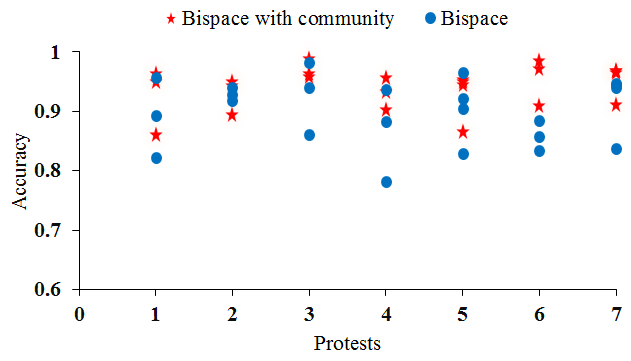
\includegraphics[width=3.5in] {figures/GBM_compare_community.png}
\caption{Performance accuracy of the bispace model for the 7
protest scenarios considered here,
with and without community structure.}
\label{fig:GBM_compare_community}
\end{figure}


\begin{itemize}
  \item \textbf{Can the bispace model simulate the propagation path?}
\end{itemize}
In addition to comparing the simulated counts of tweets over time with ground truth values, we can also compare the propagation path generated by the simulation against the actual propagation path
through the mentions network. In Fig.~\ref{fig:simulation_truth} we can
obtain a sense of the type of infection network bispace modeling creates as
compared with the actual network. The simulation produces networks with relatively accurate paths and relevant characteristics as shown in Table~\ref{table:simulation_location}. The component to which a user belongs is that of neighbors who can be reached from connected paths running along edges of the graph~\cite{newman2003structure}.


\begin{figure}[ht]
\centering
\subfigure[Simulation results]{
   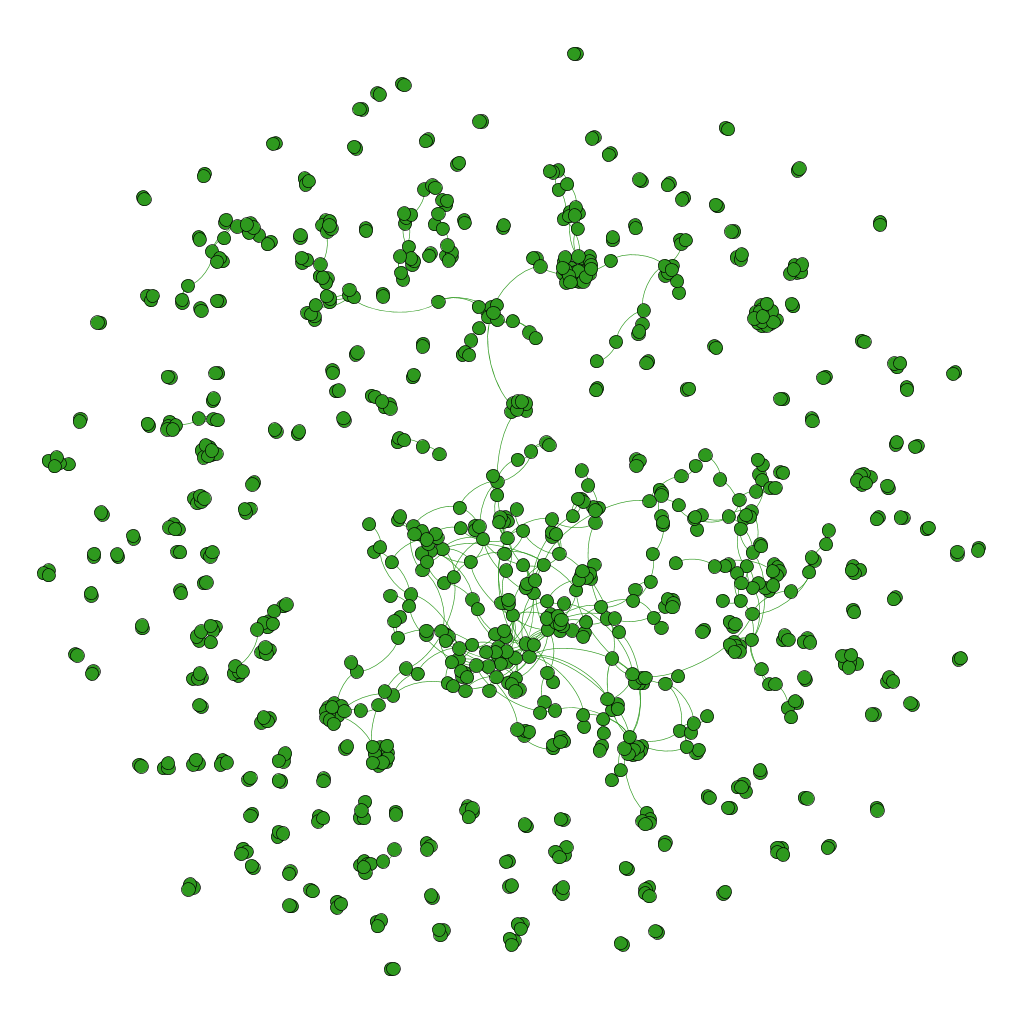
\includegraphics[width=2.5in] {figures/evaluation_simulation.png}
  \label{fig:Simulation result}
 }
 \subfigure[Truly infected nodes]{
   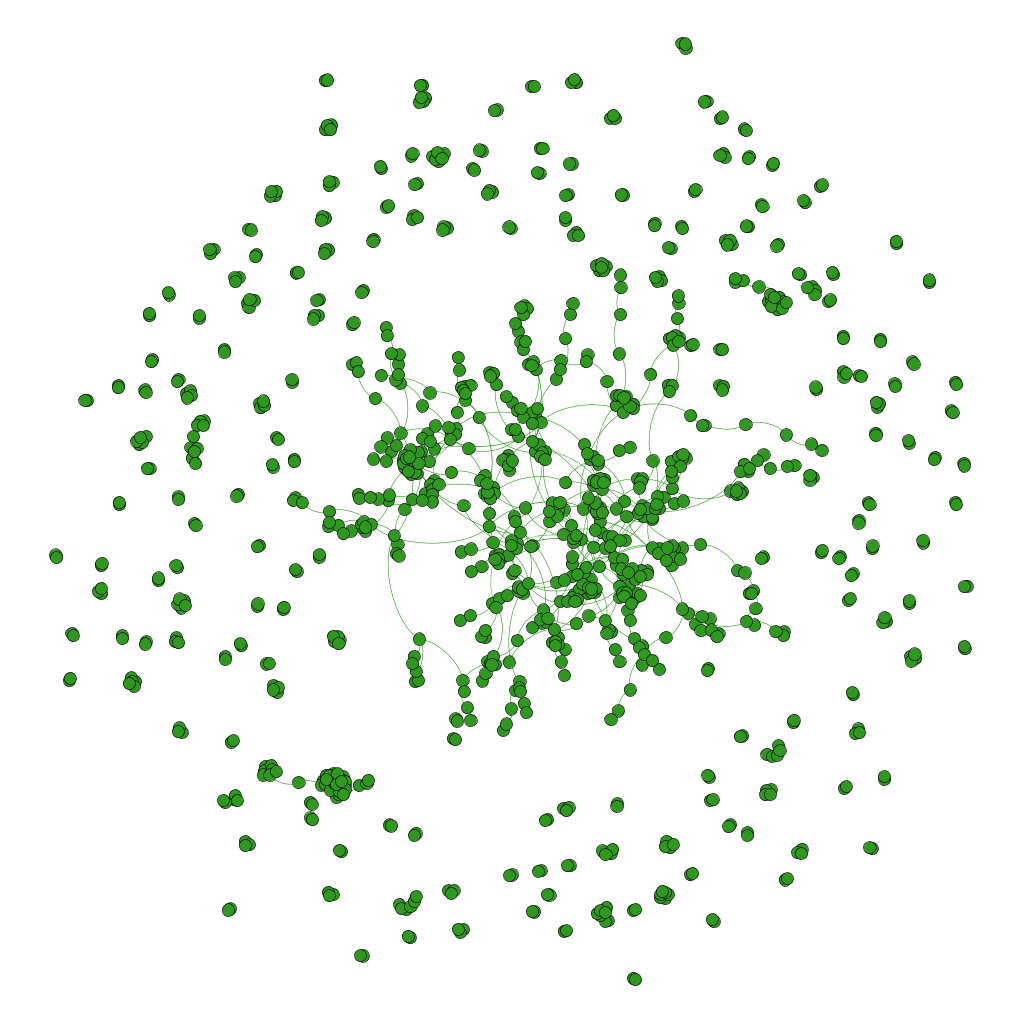
\includegraphics[width=2.5in,] {figures/true_t_mention_evaluation.png}
  \label{fig:Truly infected nodes}
 }
\caption{Bispace model simulation results compared against
ground truth infected nodes for the Mexican teacher protest events.}
\label{fig:simulation_truth}
\end{figure}




\begin{itemize}
  \item \textbf{Between the geometric Brownian model and Poisson
propagation approaches, which model
is more dominant during the simulation process?}
\end{itemize}
From Figs.~\ref{fig:1Yosoy2012may},~\ref{fig:4teacherSimulation},~\ref{fig:7ColombiaProtest}, by observing the blue dashed line (Poisson) and red dashed line (GBM), we can see that
the Poisson process shows a mild activity, while the GBM model
serves as the dominant component which can capture the moments of key
surges.
